\documentclass[12pt]{article}

\usepackage[utf8]{inputenc}
\usepackage{amsmath, amssymb, amsthm}
\usepackage{hyperref}
\usepackage{graphicx}
\usepackage{tikz}
\usepackage{multirow}
\usepackage{enumitem}
\usepackage{cancel}
\usepackage[table,x11names]{xcolor}
\usetikzlibrary{arrows}

\graphicspath{{./images/}}

\title{Lernzettel}
\author{Pascal Diller}

\setcounter{secnumdepth}{0}

\begin{document}

\maketitle
\newpage

\tableofcontents

\newpage
\section{Logik}
\begin{itemize}
    \item ''$\land$'': \textbf{Und}
    \item ''$\lor$'': \textbf{Oder}
    \item ''$\lnot$'': \textbf{Nicht} (Verneinung)
    \item $A \implies B$: $A \textbf{ impliziert} B$
    \item $A \impliedby B$: $A \text{ wird durch } B \textbf{ impliziert}$
    \item $A \Longleftrightarrow  B$: $A \text{ ist äquivalent zu } B$
    \subitem{Es gilt: $A \implies B$ und $A \impliedby B$}
    \item $\forall$: \textbf{Für alle}
    \item $\exists$: \textbf{Es existiert (mindestens) ein}
\end{itemize}

\section{Mengen}
Eine \textbf{Menge} ist eine Zusammenfassung von (mathematischen) Objekten. \\
Die Objekte in einer Menge werden als \textbf{Elemente} bezeichnet.
 
\begin{itemize}
    \item $x \in M$: x in/Element M
    \item $x \notin M$: x nicht in/Element M
\end{itemize}
\vspace{1ex}
Defintion einer Menge:
\begin{itemize}
    \item Aufzählung:
    \begin{itemize}
        \item[] $M_1 = \{0, 1, 2, 3, 5, 8, -1\}; \hspace{2ex} M_2 = \{1, 2, 3, 4, 5, \dots\}$
        \item[] Es kommt \textbf{nicht} auf die \textbf{Reihenfolge} und \textbf{nicht} auf \\ \textbf{Verdopplungen} an:
        $\{1, 3, 2, 3\} = \{3, 2, 1\} = \{1, 2, 3\}$
    \end{itemize}
    \item Beschreibung:
    \[M_3 = \{x \in \mathbb{R} : x \geq -1 \land x \leq 1\} = [-1, 1]\]
\end{itemize}
\vspace{1ex}
Menge $B$ ist eine \textbf{Teilmenge} von Menge $A$, wenn für jedes $x \in A$ auch $x \in B$ gilt.
\begin{itemize}
    \item $A \subset B$ (''$A$ ist eine Teilmenge von $B$'')
    \item $A \supset B$ (''$B$ ist eine Teilmenge von $A$'')
\end{itemize}
\vspace{1ex}
Mengenoperationen:
\begin{itemize}
    \item \textbf{Vereinigung} der Mengen $A$ und $B$
    \subitem{$A \cup B = \{x : x \in A \lor x \in B\}$ (''A vereinigt B'')}
    \item \textbf{Durchschnitt} der Mengen $A$ und $B$
    \subitem{$A \cap B = \{x : x \in A \land x \in B\}$} (''A geschnitten B'')
    \item \textbf{Differenzmenge} der Mengen $A$ und $B$
    \subitem{$A \setminus B = \{x : x \in A \land x \notin B\}$} (''A ohne B'')
\end{itemize}
\vspace{1ex}
\textbf{Kartesisches Produkt:} \\
sei $n \in \mathbb{N}$ und seien $X_1, \dots, X_n$ Mengen, dann ist
\[X_1 \times \dots \times X_n = \{(x_1, \dots, x_n) : x_i \in X_i, \text{ für } i = 1,\dots,n\}\]
die Menge der n-\textbf{Tupel} mit $i$-ter Koordinate $x_i$ in $X_i$ für $i = 1,\dots,n$. \\
\newline
\textbf{Potenzmenge:} \\
Die Menge aller Teilmengen einer Menge $X$ heißt Potenzmenge von $X$ und wird mit $\mathcal{P(X)}$ bezeichnet:
\[\mathcal{P}(X) = \{Y: Y \subset X\}\]
Es gilt immer: $\emptyset \in \mathcal{P}(X)$ und $X \in \mathcal{P}(X)$.\\
Beispiel: Sei $X = \{1, 2, 3\}$. Dann ist \[\mathcal{P}(X) = \{\emptyset, \{1\}, \{2\}, \{3\}, \{1, 2\}, \{1, 3\}, \{2. 3\}, \{1, 2, 3\}\}\]
Sei $P$ eine Menge bestehend aus Mengen. Dann steht
\[\bigcup_{Y \in P} Y = \{y: \text{ es gibt } Y \in P \text{ so dass } y \in Y\}\]
für die (möglicherweise unendliche) Vereinigung aller Mengen in $P$. \\
\newline
Partitionen: \\
Sei $X$ eine Menge. Eine Partition von $X$ ist eine Teilmenge $P \in \mathcal{P}(X) \setminus \{\emptyset\}$ sodass
\begin{itemize}
    \item für alle $Y,Z \in P$ mit $Y \neq Z, Y \cap Z = \emptyset$ ($Y$ und $Z$ sind disjunkt).
    \item $\bigcup_{Y \in P} Y = X$. 
\end{itemize}
Definierte Mengen:
\begin{itemize}
    \item Leere Menge: $\emptyset = \{\}$
    \item Natürliche Zahlen: $\mathbb{N} = \{1, 2, 3, 4, 5, 6, 7, 8, 9, 10, \dots\}$ ($0 \notin \mathbb{N}$)
    \item Ganze Zahlen: $\mathbb{Z} = \{0, 1, -1, 2, -2, 3, -3, 4, -4, \dots\}$
    \item Rationale Zahlen: $\mathbb{Q} = \left\{\frac{p}{q} : p,q \in \mathbb{Z}, q \neq 0\right\}$
    \item Relle Zahlen: $\mathbb{R}$, Menge aller \textbf{rellen Zahlen}, die man \textbf{nicht abzählen} kann
\end{itemize}
Es gilt: $\mathbb{N} \in \mathbb{Z} \in \mathbb{Q} \in \mathbb{R}$

\section{boolesche Algebra}
Als eine \textbf{boolesche Algebra} bezeichnet man eine Menge $V = \{a,b,c,\dots\}$, auf der zwei zweistellige Operationen $\oplus$ und $\otimes$ derart definiert sind, dass durch ihre Anwendung auf Elemente aus $V$ wieder Elemente aus V enstehen (Abgeschlossenheit).\\
\newline
\textbf{Abgeschlossenheit:} für alle $a,b \in V$ gilt: \[a \otimes b \in V \]\[ a \oplus b \in V\]
\newpage
Zudem müssen die vier \textbf{Huntingtonischen Axiome} gelten:
\begin{itemize}
    \item H1: \textbf{Kommutativgesetz}
        \[a \otimes b = b \otimes a\]
        \[a \oplus b = b \oplus a\]
    \item H2: \textbf{Distributivgesetz}
        \[a \otimes (b \oplus c) = (a \otimes b) \oplus (a \otimes c)\]
        \[a \oplus (b \otimes c) = (a \oplus b) \otimes (a \oplus c)\]
    \item H3: \textbf{Neutrale Elemente} \\ Es existieren zwei Elemente $e,n \in V$, so dass gilt: \\
        \begin{align*}
            a \otimes e &= a \quad &(\text{$e$ wird \textbf{Einselelement} genannt})\\
            a \oplus n &= a \quad &(\text{$n$ wird \textbf{Nullelement} genannt})
        \end{align*}
    \item H4: \textbf{Inverse Elemente} \\ Für jedes $a \in V$ existiert ein Element $a^{-1} \in V$, so dass gilt: \\
        \[a \otimes a^{-1} = n\]
        \[a \oplus a^{-1} = e\]
\end{itemize}
\subsection{Schaltalgebra}
Die Schaltalgebra $(\{0,1\}, \land, \lor)$ ist eine spezielle boolesche Algebra. 0 und 1 können als die logischen Werte wahr und falsch interpretieren. \\
Es gelten die vier Huntingtonischen Axiome: \\
\newline
\begin{tabular}{l l l}
    (H1) & Kommutativgesetz & $a \lor b = b \lor a$ \\
    & & $a \land b = b \land a$ \\
    (H2) & Distributivgesetz & $a \land (b \lor c) = (a \land b) \lor (a \land c)$ \\
    & & $a \lor (b \land c) = (a \lor b) \land (a \lor c)$ \\
    (H3) & Neutrale Elemente & $a \land 1 = a$ \\
    & & $a \lor 0 = a$ \\
    (H4) & Invere Elemente & $a \land \neg a = 0$ \\
    & & $a \lor \neg a = 1$ \\
    \multicolumn{3}{l}{Es lassen sich folgende Sätze ableiten:} \\ \\
    (R1) & Assoziativgesetz & $(a \land b) \land c = a \land (b \land c)$ \\
    & & $(a \lor b) \lor c = a \lor (b \lor c)$ \\
    (R2) & Idempotenzgesetz & $a \land a = a$ \\
    & & $a \lor a = a$ \\
    (R3) & Absorptionsgesetz & $a \land (a \lor b) = a$ \\
    & & $a \lor (a \land b) = a$ \\
    (R4) & DeMorgan-Gesetz & $\neg(a \land b) = \neg a \lor \neg b$ \\
    & & $\neg(a \lor b) = \neg a \land \neg b$ \\
\end{tabular}
\subsection{boolesche Funktionen}
Eine Funktion $f: \{0,1\}^n \rightarrow \{0,1\}$ wird als boolesche Funktion bezeichnet.
\subsection{boolescher Ausdruck}
Sei $V = \{x_1, x_2, \dots, x_n\}$ eine Menge boolescher Variablen. Dann ist die Menge der booleschen Ausdrücke wie folgt definiert: \\
\begin{itemize}
    \item $0,1,x_i$ sind boolesche Ausdrücke.
    \item Ist $\Phi$ ein boolescher Ausdruck, dann ist auch $\neg \Phi$ ein boolescher Ausdruck.
    \item Wenn $\Phi$ und $\Psi$ boolesche Ausdrücke sind, dann sind auch $\Phi \land \Psi$ und $\Phi \lor \Psi$ boolesche Ausdrücke.
    \item Ist $\Phi$ ein boolescher Ausdruck, dann ist auch $(\Phi)$ ein boolescher Ausdruck.
\end{itemize}
\subsection{Äquivalenz boolescher Ausdrücke}
Zwei boolesche Ausdrücke $\Phi$ und $\Psi$ sind äquivalent, falls sie dieselbe Funktion repräsentieren. \\ 
Sie sind genau dann äquivalent, wenn für alle Variablenbelgungen $x_1, \cdots, x_n$ die folgende Beziehung gilt:
\[\Phi(x_1,\cdots,x_n) = \Psi(x_1,\cdots,x_n)\]
\subsubsection{Tautologie}
Ein boolescher Ausdruck, der immer wahr ist, wird als \textbf{Tautologie} bezeichnet.\\
Das heißt zwei boolesche Ausdrücke $A$ und $B$ sind äquivalen, wenn $A \leftrightarrow B$ eine Tautologie ist.
\subsubsection{Vollständiges Operatorensystem}
$M$ sei eine beliebige Menge von Operatoren. $M$ ist ein \textbf{vollständiges Operatorensystem}, wenn sich jede boolesche Funktion auch durch einen Ausdruck bescreiben lässt, in dem neben den Variablen $x_1, \cdots, x_n$ ausschließlich Operatoren aus $M$ vorkommen.
\section{Normalformen}
Sei $f(x_1, \dots, x_n)$ eine beliebige $n$-stellige boolesche Funktion. \\
Ein \textbf{Minterm} ist jeder Ausdruck der Form
\[\hat{x}_1 \land \dots \land \hat{x}_n \text{ mit } \hat{x}_i \in \{\overline{x}_i, x_i\}\]
Ein \textbf{Maxterm} ist jeder Ausdruck der Form
\[\hat{x}_1 \lor \dots \lor \hat{x}_n \text{ mit } \hat{x}_i \in \{\overline{x}_i, x_i\}\]
Ein \textbf{Literal} ist der Teilausdruck $\hat{x}_i$, der entweder aus einer negierten oder einer unnegierten Variablen besteht.
\subsection{Kanonische Normalformen}
Eine kanonische Normalform ist eine \textbf{eindeutige Darstellung} mit UND, ODER und NICHT. \\
\begin{itemize}
    \item kanonische \textbf{disjunktive Normalform (DNF)}
        \subitem \hbox{Die Disjunktion (Verbinden mit ODER) von Mintermen der Funktion}
        \subitem \vbox{Die \textbf{nicht kanonische} Form ist eine Disjunktion beliebiger konjunktiv \\ verknüpfter boolescher Ausdrücke.}
    \item kanonische \textbf{konjuntive Normalform (KNF)}
        \subitem \hbox{Die Konjunktion (Verbinden mit UND) von Maxtermen der Funktion}
        \subitem \vbox{Die \textbf{nicht kanonische} Form ist eine Konjunktion beliebiger disjuntiv verknüpfter boolescher Ausdrücke.}
\end{itemize}
Es wird \textbf{ausschließlich} die \textbf{kanonische Form} behandelt und deswegen das Wort kanonisch häufig wegelassen.
\subsection{Konstruktion der Normalformen}
\subsubsection{DNF}
Es werden für jede \textbf{Einszeile} in der Wahrheitstabelle der Funktion ein \textbf{Minterm} konstruiert, der für genau diese Variablenbelgungen \textbf{1} wird. \\
Diese Minterme werden dann disjunktiv ($\lor$) verknüpft.
\subsubsection{KNF}
Es werden für jede \textbf{Nullzeile} in der Wahrheitstabelle der Funktion ein \textbf{Maxterm} konstruiert, der für genau diese Variablenbelgungen \textbf{0} wird. \\
Diese Maxterme werden dann mit konjunktiv ($\land$) verknüpft. \\
\newline
Beispiel:
\begin{center}
    \begin{tabular}{|c c c|c|l|l|}
        \hline
        $a$ & $b$ & $c$ & $f(a,b,c)$ & relative Minterme & relative Maxterme \\
        \hline
        0 & 0 & 0 & 1 & $\overline{a} \land \overline{b} \land \overline{c}$ & \\
        0 & 0 & 1 & 0 & & $a \lor b \lor \overline{c}$ \\
        0 & 1 & 0 & 0 & & $a \lor \overline{b} \lor c$ \\
        0 & 1 & 1 & 1 & $\overline{a} \land b \land c$ & \\
        1 & 0 & 0 & 1 & $a \land \overline{b} \land \overline{c}$ & \\
        1 & 0 & 1 & 0 & & $\overline{a} \lor b \lor \overline{c}$ \\
        1 & 1 & 0 & 0 & & $\overline{a} \lor \overline{b} \lor c$ \\
        1 & 1 & 1 & 1 & $a \land b \land c$ & \\
        \hline
    \end{tabular}
\end{center}
$f_{\text{DNF}}(a,b,c) = (\overline{a} \land \overline{b} \land \overline{c}) \lor (\overline{a} \land b \land c) \lor (a \land \overline{b} \land \overline{c}) \lor (a \land b \land c)$ \\
$f_{\text{KNF}}(a,b,c) = (a \lor b \lor \overline{c}) \land (a \lor \overline{b} \lor c) \land (\overline{a} \lor b \lor \overline{c}) \land (\overline{a} \lor \overline{b} \lor c)$
\subsection{Minimierung}
\subsubsection{KV-Diagramm}
Ein KV-Diagramm ist eine andere Form der Wahrheitstabelle. \\
Ausgangspunkt mit einer Variablen: \\
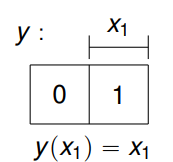
\includegraphics[scale=0.5]{image.png} \\
Erweitert wird mit einer abwechselnd horizontalen und vertikalen Spieglung. \\
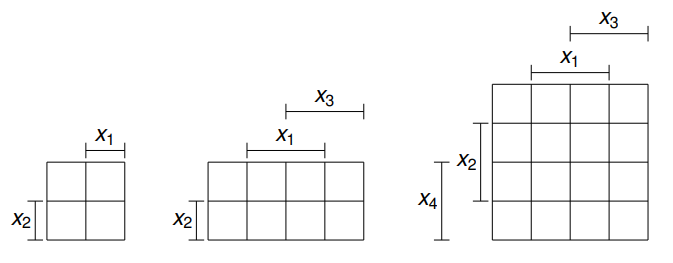
\includegraphics[scale=0.5]{image2.png} \\
Beispiel: $f(a,b,c) = (\neg a \land b) \lor (b \land c) \lor (\neg a \land \neg b \land c)$ \\
\begin{tabular}{l r}
    Wahrheitstabelle: & Es ergibt sich folgendes KV-Diagramm \\
    \begin{tabular}{c|c c c|c}
        & a & b & c & f \\ \hline
        0: & 0 & 0 & 0 & 0 \\
        1: & 0 & 0 & 1 & 1 \\
        2: & 0 & 1 & 0 & 1 \\
        3: & 0 & 1 & 1 & 1 \\
        4: & 1 & 0 & 0 & 0 \\
        5: & 1 & 0 & 1 & 0 \\
        6: & 1 & 1 & 0 & 0 \\
        7: & 1 & 1 & 1 & 1
    \end{tabular} & 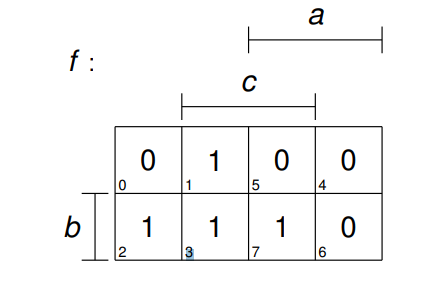
\includegraphics[scale=0.55]{image3.png} \\
\end{tabular} \\
\newline
Jedes 1-Feld entspricht einem Minterm, jedes 0-Feld einem Maxterm. \\
\newline
Gegeben seien zwei Belegungen der Variablen $x_1, \dots, x_n$. \\
Die Variable $x_i$ heißt \textbf{gebunden}, falls sie in beiden Belegungen den gleichen Wert hat. \\
Die Variable $x_i$ heißt \textbf{frei}, falls sie in beiden Belegungen ein unterschiedlichen Wert hat. \\
Zwei Variablenbelgungen heißen \textbf{benachbart}, wenn sie sich in genau einer freien Variablen unterscheiden. \\
\newline
Beispiel für benachbarte Variablenbelgungen: \\
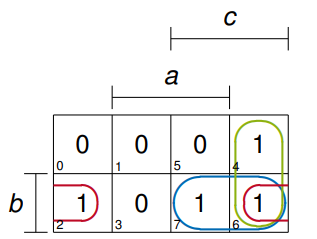
\includegraphics[scale=0.6]{image4.png} \\
Benachbarte Blöcke können ebenfalls zusammengefasst werden.
\newpage
\subsubsection{Implikanten}
\textbf{Implikant:} \\
Ein konjunktiv verknüpfter Term, der einen Block von $2^k$ Einsen beschreibt. (Implikant $k$-ter Ordnung). \\
\newline
\textbf{Primimplikant:} \\
Der Implikant zu einem nicht vergrößerbaren Eins-Block ist ein Primimplikant. \\
\newline
\textbf{Kernprimimplikant:} \\
Primimplikant, welcher mindestens eine Eins abdeckt, die durch keinen anderen Primimplikanten abgedeckt wird. 
\subsubsection{Disjuntive Minimalform über das KV-Diagramm}
\begin{enumerate}
    \item KV-Diagramm erstellen
    \subitem 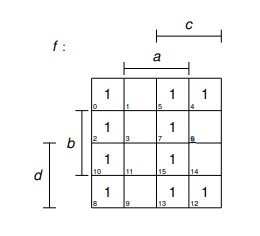
\includegraphics{image5.png}
    \item Primimplikanten bestimmen
    \subitem 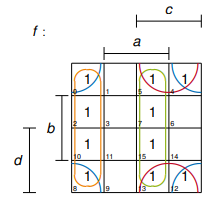
\includegraphics{image6.png}
    \item eine minimale vollständige Überdeckung finden
    \subitem Mit Kernprimimplikanten beginnen
    \subsubitem \textcolor{orange}{$\overline{a} \land \overline{b}$}, \textcolor{green}{$a \land c$}
    \subitem \vbox{Mit möglichst wenigen Primimplikanten fortfahren, bis alle 1en überdeckt sind}
    \subsubitem \textcolor{red}{$\overline{b} \land c$}
    \item Disjunktive Minimalform ablesen
    \subitem \vbox{Primimplikanten einer minimalen vollständigen Überdeckung mit $\lor$ verknüpfen}
    \subitem $f_{\text{DMF}}(a,b,c,d) = (\overline{a} \land \overline{c}) \lor (a \land c) \lor (\overline{b} \land c)$
\end{enumerate}
\subsubsection{Konjuntive Minimalform über das KV-Diagramm}
\begin{enumerate}
    \item KV-Diagramm erstellen
    \item Primimplikanten der Null-Blöcke bestimmen
    \item eine minimale vollständige Überdeckung finden
    \item Konjuntive Minimalform ablesen
    \subitem \vbox{Es werden die Variablen, die von dem Block nicht überdeckt werden disjunktiv verknüpft}
    \subitem 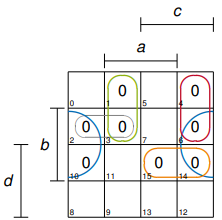
\includegraphics{image7.png}
    \subitem \textcolor{blue}{$a \lor \neg \overline{b}$}, \textcolor{green}{$\overline{a} \lor c \lor d$}, \textcolor{red}{$a \lor \overline{c} \lor d$}, \textcolor{orange}{$\overline{b} \lor \overline{c} \lor \overline{d}$}
\end{enumerate}

\section{Relationen}
Eine \textbf{(binäre) Relation} zwischen zwei Mengen $X$ und $Y$ ist eine Teilmenge
\[\text{R} \subset X \times Y\]
Im Falle $X = Y$ sprechen wir von einer Relation auf X. \\
$x \in X$ steht in Relation zu $y \in Y$ genau dann wenn $(x, y) \in \text{R}$. \\
Auch geschrieben: $x\:\text{R}\:y$ oder $x \sim_{\text{R}} y$ für $(x, y) \in \text{R}$ und $x\:\cancel{\text{R}}\:y$ oder $x \cancel{\sim}_{\text{R}} y$ für $(x,y) \notin \text{R}$. \\ \newline
Seien $X, Y$ und $Z$ Mengen und R $\subset X \times Y$, S $\subset Y \times X$ Relationen.
\begin{itemize}
    \item Die zu R \textbf{inverse Relation} ist \[\text{R}^{-1} = \{(y,x) \in Y \times X : (x, y \in \text{R})\}\]
    \item Die Verkettung von R und S ist \[\text{S} \circ \text{R} = \{(x,z) \in X \times Z : \text{es gibt } y \in Y \text{ mit } (x,y) \in \text{R und } (y,z) \in \text{S}\}\]
\end{itemize}
Eine binäre Relation R auf der Menger $X$ heißt:
\begin{itemize}
    \item \textbf{relfexiv}, wenn $x\:\text{R}\:x$ für alle $x \in X$.
    \item \textbf{symmetrisch}, wenn für alle $x, y \in X$ aus $x\:\text{R}\:y$ stets $y\:\text{R}\:x$ folgt.
    \item \textbf{antisymmetrische}, wenn für alle $x, y \in X$ aus $x\:\text{R}\:y$ und $y\:\text{R}\:x$ stets $x = y$ folgt.
    \item \textbf{asymmetrisch}, wenn für alle $x, y \in X$ aus $x\:\text{R}\:y$ stets $y\:\cancel{R}\:x$ folgt.
    \item \textbf{transitiv}, wenn für alle $x, y, z \in X$ aus $x\:\text{R}\:y$ und $y\:\text{R}\:z$ stets $x\:\text{R}\:z$ folgt.
\end{itemize}
\subsection{Äquivalenzrelationen}
Sei $X$ eine nicht leere Menge. Eine Relation R auf $X$ die relfexiv, symmetrisch und transitiv ist, heißt \textbf{Äquivalenzrelationen}. Für $x \in X$ nennt man die Menge
\[[x]\sim_{\text{R}} = \{y \in X : x\:\text{R}\:y\}\]
die \textbf{Äquivalenzklasse} von $x$. Man nennt $x$ und jedes andere Element aus $[x]\sim_{\text{R}}$ einen \textbf{Vertreter} oder \textbf{Repräsentanten} dieser Äquivalenzklasse. \\
\newline
Sei $X$ eine Menge und $\sim$ eine Äquivalenzrelation auf $X$. Ein \textbf{Vertretersystem} ist eine Teilmenge von $X$, die für jede Äquivalenzklasse genau ein Element enthält.
\subsection{Ordnungsrelationen}
Sei $X$ eine Menge. Eine \textbf{Ordnung} auf $X$ ist eine reflexive, antisymmetrische und transitive Relation. Eine \textbf{strikte Ordnung} auf X ist eine asymmetrisch und transitive Relation. Wir nennen eine (strikte) Ordnung $\preceq$ \textbf{total}, wenn je zwei Elemente vergleichbar sind: 
\[\text{für alle } x,y \in X \text{ gilt } x \preceq y \text{ oder } y \preceq x\]
Ansonsten nennen wir sie \textbf{partiell}.
\subsection{Hüllen}
Sei R eine Relation auf der Menge $X$. Wir definieren:
\begin{itemize}
    \item Für $n \in \mathbb{N}_0$ \[R^n = \begin{cases}
        \text{I}_X & n = 0 \\
        \text{R} \circ \text{R}^{n-1} & n \geq 1 \\
    \end{cases}\] Es gilt, dass R$^1 = $ R
    \item Die \textbf{transitive Hülle} von R ist \[\text{R}_{\text{trans}} = \bigcup_{n\in\mathbb{N}} \text{R}^n\]
    \item Die \textbf{reflexive Hülle} von R ist \[\text{R}_{\text{refl}} = \text{R} \cup \text{I}_X\]
    \item Die \textbf{symmetrische Hülle} von R ist \[\text{R}_{\text{sym}} = \text{R} \cup \text{R}^{-1}\]
\end{itemize}

\newpage
\section{Vollständige Induktion}
Das \textbf{Prinzip der vollständigen Induktion} ist ein Beweisverfahren, mit dem man Aussagen $A(n)$ beweisen kann, die von $n \in \mathbb{N}_0$ abhängen.
\subsection{Idee der vollständigen Induktion}
Zu zeigen sei die Aussage $A(n)$ für alle $n \in \mathbb{N}_0$ mit $n \geq n_0$ für ein $n_0 \in \mathbb{N}$. \\
Angenommen, man kann zeigen, dass $A(n_0)$ gilt, und weiter kann man beweisen, dass $A(n+1)$ gilt, wenn man voraussetzt, dass $A(n)$ gilt, d.h. die Implikation $A(n) \implies A(n + 1)$ ist für alle $n \in \mathbb{N}, n \geq n_0$ gültig. \\
Dann gilt $A(n)$ für alle $n \in \mathbb{N}$ mit $n \geq n_0$.\\
\subsection{Beweis durch vollständige Induktion}
\begin{enumerate}
    \item \textbf{Induktionsanfang (I.A.)}: Es gibt ein $n_0 \in \mathbb{N}_0$, sodass $A(n_0)$ wahr ist.
    \item \textbf{Induktionsvoraussetzung (I.V.)}: Annahme: $A(n)$ ist wahr (für ein $n \geq n_0$).
    \item \textbf{Induktionsschluss (I.S.)}: Zeige: $A(n) \implies A(n+1)$.
\end{enumerate}

\newpage
\section{Abbildungen}
Eine \textbf{Abbildung} $f: X \to Y$ besteht aus:
\begin{itemize}
    \item einer Menge X, der \textbf{Definitionsbereich} von $f$;
    \item einer Menge Y, der \textbf{Wertebereich} von $f$;
    \item einer \textbf{Vorschrift}, die jedem $x \in X$ eindeutig ein $y \in Y$ zuordnet.
\end{itemize}
Notation: $f: X \to Y, x \mapsto f(x)$ \\ 
\newline
\hbox{Seien $X, Y$ Mengen, $f: X \to Y$ eine Abbildung und $x \in X, y \in Y$ sodass $f(x)=y$.} \\
Dann ist $y$ das \textbf{Bild} von $x$ und $x$ ein \textbf{Urbild} von $y$.\\
Für eine Teilmenge $X_0 \subset X$ ist
\[f(X_0) := \{y \in Y: \text{ es gibt } x \in X_0 \text{, sodass } f(x)=y\} \subset Y\]
das \textbf{Bild} von $X_0$ und für eine Teilmenge $Y_0 \subset Y$ ist
\[f^{-1}(Y_0) := \{x \in X : f(x) \in Y_0\} \subset X\]
das \textbf{Urbild} von $Y_0$. \\ 
\newline
Seien $X$ und $Y$ Mengen und $f: X \to Y$ eine Abbildung.
\begin{itemize}
    \item[] $f$ ist \textbf{injektiv} falls aus $x_1,x_2 \in X$ mit $f(x_1) = f(x_2)$ stets $x_1 = x_2$ folgt.
        \subitem{''zu jedem y höchstens 1 x-Wert''}
    \item[] $f$ ist \textbf{surjektiv} falls es für jedes $y \in Y$, ein $x \in X$ existiert so dass $f(x) = y$.
        \subitem{''zu jedem y mindestens 1 x-Wert''}
    \item[] $f$ ist \textbf{bijektiv} falls $f$ injektiv und surjektiv ist.
\end{itemize}
Seien $X, Y, Z$ Mengen und $f: X \to Y$ und $g: Y \to Z$ Abbildungen.\\
Die \textbf{Komposition} oder \textbf{Verknüpfung} von $f$ und $g$ ist die\\
Abbildung $g \circ f: X \to Z$, definiert durch $(g \circ f)(x)=g(f(x))$.

\section{Reelle Funktionen}
Sei $M$ eine Menge. Eine Abbildung $f: M \to \mathbb{R}$ heißt Funktion. \\
\newline
Für Funktionen $f,g: M \to \mathbb{R}$ sind $f+g, f \cdot g, \frac{f}{g}$ defintiert durch
\begin{itemize}
    \item $(f+g)(x) := f(x) + g(x)$ für $x \in M$
    \item $(f \cdot g)(x) := f(x) \cdot g(x)$ für $x \in M$
    \item $\frac{f}{g}(x) := \frac{f(x)}{g(x)}$ für $x \in M \setminus \{x \in M : g(x) = 0\}$ 
    \item[] \textbf{''punktweise''} Entsprechend 
    \item $|f|(x) := |f(x)|$, max$\{f,g\}(x) :=$ max$\{f(x), g(x)\}$, \\min$\{f,g\}(x) :=$ min$\{f(x),g(x)\}$ für $x \in M$
    \item $f \leq g$ genau dann wenn $f(x) \leq g(x)$ für alle $x \in M$.
\end{itemize}
Für eine Abbildung $f : N \to M$ mit $N,M \subset \mathbb{R}$ wird $f^{-1}:M \to N$ als \textbf{Umkehrfunktion} von $f$ bezeichnet. \\
(!!! $f^{-1} \neq x \mapsto \frac{1}{f(x)}$ für $x \in M$)
\subsection{Funktionsgraphen}
Seien $M$ eine Menge und $f: M \to \mathbb{R}$ eine Funktion. Dann ist der \textbf{Graph} von $f$
\[\Gamma(f) := \{(x,f(x)): x \in M\} \subset M \times \mathbb{R}\]
\subsubsection{Intervalle}
Definitionsbereiche von reellen Funktionen sind oft Intervalle. 
\begin{itemize}
    \item beschränkte Intervalle für $a, b \in \mathbb{R}, a \leq b$
    \begin{align*}
        [a,b] &:= \{x \in \mathbb{R} : a \leq x \leq b\} \text{ ''abgeschlossen'', ''kompakt''} \\
        (a,b) &:= \{x \in \mathbb{R} : a < x < b\} \text{ ''offen''} \\
        [a,b) &:= \{x \in \mathbb{R} : a \leq x < b\} \text{ ''halboffen''} \\
        (a,b] &:= \{x \in \mathbb{R} : a < x \leq b\} \text{ ''halboffen''} 
    \end{align*}
    \item[] mit $[a,b] = [a, a] = {a}$ für $a = b$ und $(a,b) = [a,b) = (a,b] = \emptyset$ für $a = b$.
    \item unbeschränkte Intervalle für $a \in \mathbb{R}$
    \begin{align*}
        [a,\infty) &:= \{x \in \mathbb{R}: a \leq x\} \text{ ''abgeschlossen''} \\
        (-\infty, a] &:= \{x \in \mathbb{R}: x \leq a\} \text{ ''abgeschlossen''} \\
        (a,\infty) &:= \{x \in \mathbb{R}: a < x\} \text{ ''offen''} \\
        (-\infty, a) &:= \{x \in \mathbb{R}: x < a\} \text{ ''offen''} 
    \end{align*}
\end{itemize}
\subsection{Beschränkte Mengen und Funktionen}
Eine Menge $M \subset \mathbb{R}$ heißt
\begin{itemize}
    \item \textbf{nach oben beschränkt} genau dann wenn $\exists C \in \mathbb{R} \forall x \in M : x \leq C$
        \subitem $C$ heißt \textbf{obere Schranke}
        \subitem Falls $M \subset \mathbb{R}$ ein Maximum besitzt ist $M$ nach oben beschränkt.
    \item \textbf{nach unten beschränkt} genau dann wenn $\exists c \in \mathbb{R} \forall x \in M : x \leq c$
        \subitem $c$ heißt \textbf{untere Schranke}
        \subitem Falls $M \subset \mathbb{R}$ ein Minimum besitzt ist $M$ nach unten beschränkt.
    \item \textbf{beschränkt} genau dann wenn $M$ nach oben und nach unten beschränkt
\end{itemize}
Betrachte die Funktion $f: M \to \mathbb{R}$
\begin{itemize}
    \item $f$ heißt nach \textbf{oben/unten beschränkt} genau dann wenn $f(M)$ nach oben/unten beschränkt ist.
    \item $f$ besitzt ein \textbf{Maximum/Minimum} auf $M$ genau dann wenn $f(M)$ ein Maximum/Minimum besitzt.
    \item Ein Punkt $x_0 \in M$ mit 
        \subitem $f(x_0) =$ max$f(M) =: \underset{x \in M}{\text{max}} f(x)$ heißt \textbf{Maximalstelle} von $f$,
        \subitem $f(x_0) =$ min$f(M) =: \underset{x \in M}{\text{min}} f(x)$ heißt \textbf{Minimalstelle} von $f$.
    \item Ein Punkt $x_0 \in M$ heißt \textbf{Extremstelle} von $f$, wenn $x_0$ eine Maximal- oder Minimalstelle ist.
\end{itemize}
\subsection{Monotone Funktionen}
Sei $M \subset \mathbb{R}$ und $f: M \to \mathbb{R}$. Dann heißt $f$
\begin{itemize}
    \item \textbf{monoton wachsend}, falls $\forall x,y : x \leq y \to f(x) \leq f(y)$
    \item \textbf{streng monoton wachsend}, falls $\forall x,y : x < y \to f(x) < f(y)$
    \item \textbf{monoton fallend}, falls $\forall x,y : x \leq y \to f(x) \geq f(y)$
    \item \textbf{streng monoton fallend}, falls $\forall x,y : x < y \to f(x) > f(y)$
\end{itemize}
\subsection{Trigonometrische Funktionen}
Betrachte einen Winkel $\alpha$ mit Schenkeln der Länge 1 und Spitze im Ursprung $(0,0) \in \mathbb{R}^2$ \\
Wenn $\alpha > 0$, dann ist der Winkel orientiert, d.h. Die Strecke des Winkels wird \textbf{gegen den Uhrzeigersinn} gedreht.\\
Wenn $\alpha < 0$, dann ist die Strecke des Winkels \textbf{im Uhrzeigersinn} gedreht. \\
Für die Länge $x = x(\alpha)$ des Kreisbogens die Verhältnisgleichung
\[\frac{x}{2\pi} = \frac{\alpha}{360^{\circ}} \Longleftrightarrow x = x(\alpha) = \frac{\alpha \cdot 2\pi}{360^{\circ}}\]
\subsection{Sinus- und Cosinus-Funkton}
Betrachte den Vektor $(u(x),v(x))$ auf dem Einheitskreis um 0, der mit der positiven $x$-Achse den Winkel $x = x(\alpha)$ bildet. \\
Dann ist die \textbf{Cosinus-Funktion} definiert als
\[\cos(x) := u(x) \text{ für } x \in \mathbb{R}\]
und die \textbf{Sinus-Funktion} definiert als
\[\sin(x) := v(x) \text{ für } x \in \mathbb{R}\]
Es folgen wesentliche Eigenschaften von Sinus und Cosinus:
\begin{itemize}
    \item $\cos$ und $\sin$ sind $2\pi$-periodisch. Für alle $x \in \mathbb{R}$ und $k \in \mathbb{Z}$ gilt $\cos(x+2k\pi) = \cos(x)$ und $\sin(x+2k\pi) = \sin(x)$
    \item $\cos(-x) = \cos(x) \implies \cos$ ist eine \textbf{gerade} Funktion.
    \item $\sin(-x) = -\sin(x) \implies \sin$ ist eine \textbf{ungerade} Funktion.
    \item $\cos^2(x) + \sin^2(x) = 1$
    \item $|\cos(x)| \leq 1, \: |\sin(x)| \leq 1, \: |\sin(x)| \leq |x|$
\end{itemize}
Für $x,y \in \mathbb{R}$ gelten die \textbf{Additionstheoreme} 
\begin{align*}
    \cos(x \pm y) &= \cos(x) \cos(y) \mp \sin(x) \sin(y) \\
    \sin(x \pm y) &= \sin(x) \cos(y) \pm \cos(x) \sin(y) \\
\end{align*}
Spezialfälle:
\begin{align*}
    \sin \left( x + \frac{\pi}{2} \right) &= \sin(x) \underbrace{\cos\left(\frac{\pi}{2}\right)}_{=0} + \cos(x) \underbrace{\sin\left(\frac{\pi}{2}\right)}_{=1} = \cos(x) \\
    \cos \left( x - \frac{\pi}{2} \right) &= \cos(x) \underbrace{\cos\left(\frac{\pi}{2}\right)}_{=0} + \sin(x) \underbrace{\sin\left(\frac{\pi}{2}\right)}_{=1} = \sin(x) 
\end{align*}
\subsection{Tangens-Funktion}
\[\tan(x) := \frac{\sin(x)}{\cos(x)} \text{ für } x \in D := \mathbb{R} \setminus \{(k+\frac{1}{2})\pi : k \in \mathbb{Z}\}\]
Eigenschaften des Tangens:
\begin{itemize}
    \item Die Tangens-Funktion ist $\pi$-periodisch, d.h. für $k \in \mathbb{Z}$ und $x \in D$ gilt
    \[\tan(x + k\pi) = \frac{\sin(x + k\pi)}{\cos(x + k\pi)} = \frac{\sin(x) \cos(k\pi) + \cos(x) \sin(k\pi)}{\cos(x) \cos(k\pi) - \sin(x) \sin(k\pi)} = \frac{\mp \sin(x)}{\mp \cos(x)} = \tan(x).\]
    \item Die Tangens-Funktion ist ungerade, es gilt für $x \in D$
    \[\tan(-x) = \frac{\sin(-x)}{\cos(-x)} = \frac{-sin(x)}{cos(x)} = -\tan(x)\]
\end{itemize}
\subsection{Polynome}
Sei $t$ eine \underline{Variable} oder \underline{Unbestimmte}. Ein \textbf{Polynom mit Koeffizienten in $\mathbb{R}$} oder ein \textbf{Polynom über $\mathbb{R}$} ist ein formaler Ausdruck der Gestalt
\[P(t) := \sum_{k=0}^{m}a_k t^k = a_m t^m + a_{m-1} t^{m-1} + \ldots + a_1 t + a_0\]
mit $a_0, \dots, a_m \in \mathbb{R}$. Die Menge aller Polynome über $\mathbb{R}$ wird mit $\mathbb{R}[t]$ bezeichnet. Falls $a_m \neq 0$ (\textbf{Leitkoeffizient}) gilt, dann heißt $m$ der \textbf{Grad} von $P$. \\
\newline
Notation:
\begin{itemize}
    \item Wir bezeichnen mit $\deg P$ den Grad von $P$.
    \item Für das Nullpolynom $N$, bei dem alle $a_i$ Null sind, ist $\deg N := -\infty$.
    \item $\mathbb{R}_m[t] := \{ P \in \mathbb{R}[t] : \deg P \leq m \}$.
    \item Polynome von Grad 0 $(P(x) = a_0)$ sind die \textbf{konstanten Polynome}.
    \item Polynome von Grad 1 $(P(x) = a_1 x + a_0)$ sind die \textbf{linearen Polynome}.
    \item Polynome von Grad 2 $(P(x) = a_2 x^2 + a_1 x + a_0)$ sind die \textbf{quadratischen Polynome}.
\end{itemize}
Eine \textbf{Polynomfunktion} ist eine Funktion der Form $\mathbb{R} \to \mathbb{R}, x \mapsto P(x)$ für ein Polynom $P \in \mathbb{R}[t]$. \\
\newline
Seien $M \subset \mathbb{R}, x_0 \in M$ und $f: M \to \mathbb{R}$. Dann heißt $x_0$ \textbf{Nullstelle} von $f$, falls $f(x_0) = 0$ gilt. \\ 
Ein Polynom $P \in \mathbb{R}_m[x]$ vom Grad $m \in \mathbb{N}$ hat \textbf{höchstens $m$} Nullstellen.

\section{Der Euklidische Raum $\mathbb{R}^n$}
Der $n$-\textbf{dimensionale euklidische Raum} ist
\[\mathbb{R}^n = \mathbb{R} \times \dots \times \mathbb{R} = \{(\xi_1, \dots, \xi_n) | \xi_1, \dots \xi_n \in \mathbb{R}\}\]
$\mathbb{R}^0$ ist der \textbf{Nullraum}. \\
$\mathbb{R}^1$ sind die reellen Zahlen selbst. \\
$\mathbb{R}^2$ ist die euklidische Ebene. \\
Die Elemente in $\mathbb{R}^n$ heißen je nach Zusammenhang \textbf{Punkt} oder \textbf{Vektor}.
\subsection{Skalarprodukt}
Das \textbf{Skalarprodukt} zweier Vektoren $a = (\xi_i)$ und $b = (\eta_i)$ im $\mathbb{R}^n$ ist definiert als
\[a \cdot b = \xi_1 \eta_1 + \dots + \xi_n \eta_n \in \mathbb{R}.\]
Für $a,b,c \in \mathbb{R}^n$ und $t \in \mathbb{R}$ gilt: \\
\newline
\begin{tabular}{l l}
    (bilinear) & $(a+b) \cdot c = a \cdot c + b \cdot c$ und $a \cdot (b+c) = a \cdot b + a \cdot c$ \\
    & $(\lambda a) \cdot b = a \cdot (\lambda b) = \lambda(a \cdot b)$ \\
    (symmetrisch) & $a \cdot b = b \cdot a$ \\
    (positiv definiert) & $a \cdot a \geq 0$ und $a \cdot a = 0 \Leftrightarrow a = 0$
\end{tabular} \\
Das Skalarprodukt ist ebenfalls definiert als
\[a \cdot b = \cos(\alpha)\cdot||a||\cdot||b||\]
\[\Leftrightarrow \cos(\alpha) = \frac{a \cdot b}{||a|| \cdot ||b||}\]
\subsection{Norm/Länge eines Vektors}
Die \textbf{Norm} oder \textbf{Länge} von $a \in \mathbb{R}^n$ ist \[||a||= \sqrt{a \cdot a} = \sqrt{\sum {a_i}^2}\]
Seien $\lambda \in \mathbb{R}$ und $a \in \mathbb{R}^n$. Es gilt:
\[||\lambda \cdot a|| = |\lambda| \cdot ||a||\]
\[||a|| = 0 \Longleftrightarrow a = 0\]
\subsection{Lineare Gleichungssysteme}
Eine \textbf{lineare Gleichung} (über $\mathbb{R}$) ist ein Ausdruck der Form
\[\alpha_1x_1 + \dots + \alpha_nx_n = \beta\]
für die Unbekannten $x_1, \dots, x_n$ und reelle Zahlen $\alpha_i$ (\textbf{Koeffizienten}) und $\beta$. Eine \textbf{Lösung} ist ein $n$-Tupel $(\xi_1, \dots, \xi_n) \in \mathbb{R}^n$ das die Gleichung erfüllt. \\
\newline
Ein \textbf{lineares Gleichungssystem} $G$ (in $n$ Variablen) ist ein System \\
\begin{center}
    \begin{tabular}{c c c c c c c c c}
        $a_{11}x_1$ & + & $a_{12}x_2$ & + & $\dots$ & + & $a_{1n}x_n$ & = & $\beta_1$ \\ 
        $a_{21}x_1$ & + & $a_{22}x_2$ & + & $\dots$ & + & $a_{2n}x_n$ & = & $\beta_2$ \\ 
        & & $\vdots$ & & & & \\
        $a_{m1}x_1$ & + & $a_{m2}x_2$ & + & $\dots$ & + & $a_{mn}x_n$ & = & $\beta_m$ \\ 
    \end{tabular}
\end{center}
von $m$ linearen Gleichungen. Ein lineares Gleichungssystem heißt \textbf{homogen} wenn $\beta_i = 0$ für alle $i=1,\dots,m$. \\
\newline
Die eigentliche Information des linearen Gleichungssystems liegt in den \textbf{Koeffizienten} und den \textbf{Konstanten} auf der rechten Seite der Gleichung. \\
Die \textbf{augmentierte Matrix} ($(m \times n+1)$-Matrix) kodiert diese Informationen.
\[A = \begin{pmatrix}
    
    \alpha_{11} & \alpha_{12} & \dots & \alpha_{1n} & \beta_1 \\
    \alpha_{21} & \alpha_{22} & \dots & \alpha_{2n} & \beta_2 \\
    \vdots & \vdots & & \vdots & \vdots\\
    \alpha_{m1} & \alpha_{m2} & \dots & \alpha_{mn} & \beta_m
\end{pmatrix}\]
Die Koeffizienten werden in einer \textbf{Koeffizientenmatrix} $A$ ($(m \times n)$-Matrix) kodiert.
\[A = (\alpha_{ij}) = \begin{pmatrix}
    \alpha_{11} & \alpha_{12} & \dots & \alpha_{1n} \\
    \alpha_{21} & \alpha_{22} & \dots & \alpha_{2n} \\
    \vdots & \vdots & & \vdots \\
    \alpha_{m1} & \alpha_{m2} & \dots & \alpha_{mn}
\end{pmatrix}\]
\subsubsection{Lösungsmenge}
Die Lösungsmenge
\[L(G) = \left\{(\xi_1, \dots, \xi_n) \in \mathbb{R}^n: \sum_{j=1}^{n} \alpha_{ij}\xi_{j} = \beta_i \text{ für } i = 1, \dots, m\right\}\]
von einem Gleichungssystem $G$ besteht aus den $n$-Tupeln, den \textbf{Lösungen}, die alle Gleichungen von $G$ erfüllen.

\newpage
\subsection{Matrizen}
Ein Zahlenschema
\[A = (\alpha_{ij}) = \begin{pmatrix}
    \alpha_{11} & \alpha_{12} & \dots & \alpha_{1n} \\
    \alpha_{21} & \alpha_{22} & \dots & \alpha_{2n} \\
    \vdots & \vdots & & \vdots \\
    \alpha_{m1} & \alpha_{m2} & \dots & \alpha_{mn}
\end{pmatrix}\]
wird $m \times n$-\textbf{Matrix} genannt, wobei $m$ die Anzahl der \textbf{Zeilen} und $n$ die Anzahl der \textbf{Spalten} von $A$ sind.
Für eine Eintrag $\alpha_{ij}$ von $A$ ist $i$ der \textbf{Zeilenindex} und $j$ der \textbf{Spaltenindex} \\
\newline
Eine Matrix $A = (\alpha_{ij})$ heißt
\begin{itemize}
    \item \textbf{quadratisch} wenn $n = m$
    \item \textbf{Nullmatrix} wenn $\alpha_{ij} = 0, \: \forall i,j \in \mathbb{N}$
\end{itemize}
Eine quadratische Matrix heißt
\begin{itemize}
    \item \textbf{diagonal} wenn $\alpha_{ij} = 0$ für $i \neq j$
    \item \textbf{obere Dreiecksmatrix} wenn $\alpha_{ij}= 0$ für $i > j$.
    \item \textbf{untere Dreiecksmatrix} wenn $\alpha_{ij} = 0$ f+r $i < j$.
\end{itemize}

\section{Zahlensysteme}
\subsection{Binärsystem}
\begin{itemize}[leftmargin=*]
    \item[] Eine Binärzahl $b$ mit $n + 1$ Stellen hat die Form $b_n\dots b_1 b_2$ mit $b_i \in \{0,1\}$.
    \item[] Sie entspricht der Dezimalzahl $d$ mit $d = b_n \cdot 2^n + \cdots + b_1 \cdot 2^1 + b_0 \cdot 2^0$ 
    \item[] Beispiel: $1101_2 = 1 \cdot 2^3 + ^\cdot 2^2 + 0 \cdot 2^1 + 1 \cdot 2^0 = 13_{10}$
\end{itemize}
\subsubsection{Carry-Flag}
Wenn bei einer Addition oder Subtraktion ein \textbf{Übertrag in der höchsten Stelle} auftritt, wird die Carry-Flag gesetzt.
Dieser kann von nachfolgenden Befehlen aufgerufen werden.
\subsubsection{Zweierkomplement}
\begin{itemize}[leftmargin=*]
    \item[] Um \textbf{negative Zahlen} darzustellen wird der entsprechende Wert des \textbf{höchsten Bits negiert}.
    \item[] Beispiel bei 4 Bit: $1011_{2c} = 1 \cdot (-2^3) + 0 \cdot 2^2 + 1 \cdot 2^1 + 1 \cdot 2^0 = -5$
    \item[] Um von einer positiven ganzen Zahl zur negativen Zahl (oder umgekehrt) gleichen Betrags zu gelangen werden \textbf{alle Bits invertiert} und \textbf{1 zum Ergebnis addiert}.
\end{itemize}

\subsection{Hexadezimalsystem}
\begin{itemize}[leftmargin=*]
    \item[] Eine Hexadezimalzahl $h$ mit $n + 1$ Stellen hat die Form $h_n \dots h_1 h_0$ mit $h_i \in \{0, 1, 2, 3, 4, 5, 6, 7, 8, 9, A(\widehat{=}10), B(\widehat{=}11), C(\widehat{=}12), D(\widehat{=}13), E(\widehat{=}14), F(\widehat{=}15)\}$.
    \item[] Sie entspricht der Dezimalzahl $d$ mit $d = h_n \cdot 16^n + h_1 \cdot 16^1 + h_0 \cdot 16^0$.
    \item[] Beispiel: $\mathtt{5F}_{16} = 5 \cdot 16^1 + 15 \cdot 16^0 = 95_{10}$
    \item[] 4 Binärziffern lassen sich zu einer Hexadezimalzahl zusammenfassen:\\$\underbrace{1101}_{13_{10}=D_{16}} \underbrace{0011_2}_{3_{16}} = \mathtt{D3_{16}}$
\end{itemize}
\subsection{Oktalsystem}
\begin{itemize}[leftmargin=*]
    \item[] Eine Oktalzahl $o$ mit $n + 1$ Stellen hat die Form $o_n \dots o_1 o_0$ mit $o_i \in \{0, 1, 2, 3, 4, 5, 6, 7\}$
    \item[] Sie entspricht der Dezimalzahl $d$ mit $d = o_n \cdot 8^n + \cdots + o_1 \cdot 8^1 + o_0 \cdot 8^0$.
    \item[] Beispiel: $36_8 = 3 \cdot 8^1 + 6 \cdot 8^0 = 30_{10}$
    \item[] 3 Binärziffern lassen sich zu einer Oktalzahl zusammenfassen:\\$\underbrace{11}_{3_8} \underbrace{010}_{2_8} \underbrace{011_2}_{3_8} = 323_8$
\end{itemize}
\subsection{Festkommazahlen}
Eine Festkommazahl besteht aus einer \textbf{festen Anzahl von Ziffern vor und nach dem Komma}.\\ \newline
\begin{tabular}{c|c|c|c|c|c|c|c|c}
    $2^3$ & $2^2$ & $2^1$ & $2^0$ &  & $2^{-1}$ & $2^{-2}$ & $2^{-3}$ & $2^{-4}$ \\ \hline
    1 & 1 & 0 & 1 & . & 0 & 1 & 0 &1
\end{tabular}
\subsection{Gleitkommazahlen: IEEE 754}
3 Formate:
\begin{itemize}
    \item Single Precision: 32 Bit
    \item Double Precision: 64 Bit
    \item Extended Precision: 80 Bit
\end{itemize}
Basiert auf der wissenschaftlichen Notation.
\subsubsection{Aufbau}
\begin{tabular}{@{}l l}
    Single Precision: &
    \begin{tabular}{|c|c|c|}
        \hline
        1 Bit Vorzeichen & 8 Bit Exponent & 23 Bit normalisierte Mantisse\\
        \hline
    \end{tabular} \\
    Double Precision: &
    \begin{tabular}{|c|c|c|}
        \hline
        1 Bit Vorzeichen & 11 Bit Exponent & 52 Bit normalisierte Mantisse\\
        \hline
    \end{tabular}
\end{tabular} \\
\newline
Vorzeichen: $0 = +$; $1 = -$ \\
\newline
Exponent: wird gespeichert, indem man den festen Biaswert (127:SP, 1023:DP) addiert. \\
\newline
Die Mantisse beginnt mit einem ''Hidden Bit'' (immer 1).
\subsubsection{Dezimal zu IEEE 754}
Beispiel: -62.058
\begin{enumerate}
    \item Vorzeichen Bit bestimmen
    \subitem{Vorzeichen Bit = 1}
    \item Zu pur Binär umwandeln
    \subitem{$62.058_{10} = 111110.10010100_2$}
    \item Normalisieren für Mantisse und Exponent (ohne Bias)
    \subitem{$111110.10010100_2 = 1.1111010010100_2 \cdot 2^5$}
    \item Exponent mit Bias bestimmen
    \subitem{$5 + 127 = 132_{10} = 10000100_2$}
    \item Führende 1 der Mantisse abschneiden
    \subitem{$1.1111010010100_2 \rightarrow 1111010010100_2$}
    \item Zusammenfügen
    \subitem{$-62.058_{10} = \underbrace{1}_{\substack{\text{Vorzeichen}\\ \text{Bit}}} \underbrace{10000100}_{\text{Exponent}} \underbrace{1111010010100}_{\text{Mantisse}}$}
\end{enumerate}
\subsubsection{IEEE 754 zu Dezimal}
Beispiel: $01000010011010100000000000000000$
\begin{enumerate}
    \item Vorzeichen bestimmen
    \subitem{Vorzeichen: $+$}
    \item Exponent bestimmen (Bias muss abgezogen werden)
    \subitem{$10000100_2 - 127_{10} = 132_{10} - 127_{10} = 5_{10}$}
    \item Mantisse bestimmen
    \subitem{
        \begin{tabular}{|c|c|c|c|c|c|}
            $\frac{1}{2}$ & $\frac{1}{4}$ & $\frac{1}{8}$ & $\frac{1}{16}$ & $\frac{1}{32}$ & $\frac{1}{64}$ \\ \hline
            1 & 1 & 0 & 1 & 0 & 1
        \end{tabular}
    }
    \subitem{$\frac{1}{2} + \frac{1}{4} + \frac{1}{16} + \frac{1}{64} = \frac{53}{64} = 0.828125$}
    \item 1 zur Mantisse addieren (Hidden Bit) und Vorzeichen einrechnen
    \subitem{1.828125}
    \item Ergebnis berechnen
    \subitem{$1.828125 \cdot 2^5 = 58.5_{10}$}
\end{enumerate}
\section{Fehlererkennung}
\subsection{Redundanzen}
Eine Einheite von $n$ Datenbits und $k$ Redundanzbits nennt man \textbf{Codewort}.\\
Die \textbf{Länge} eines Codeworts ist insgesammt $n+k$.\\
Die Menge aller gültigen Codewörter nennt man \textbf{Code}.
\subsection{Hamming-Distanz}
Die Hamming Distanz zweier Codewörter ist gegeben als die Anzahl der Bitpositionen, in denen sie sich unterscheiden. \\
\indent Beispiel: $11110000$ und $11001100 \implies$ Hamming-Distanz beträgt 4 \\ \newline 
Die Hamming Distanz eines Codes ist die kleinste Hamming-Distanz zweier Codewörter \\
\indent Beispiel: $\{1100, 0011, 1111\} \implies$ Hamming-Distanz beträgt 2 \\ \newline
$c$-Bit Fehler können erkannt werden, wenn die Hamming-Distanz $c+1$ beträgt.
$c$-Bit Fehler können korrigiert werden, wenn die Hamming-Distanz $2c+1$ beträgt.
\subsection{Parität}
Durch Hinzufügen eines \textbf{Paritätsbits} wird ein Code mit Hamming-Distanz 2 erzeugt.
\begin{itemize}
    \item[] Das Paritätsbit wird gesetzt sodass die Gesamtzahl der 1en...
    \item[] ... gerade ist
    \subitem{$\underbrace{00100101}_{Datenbits} \underbrace{1}_{\text{Paritätsbit}}$}
    \item[] ... ungerade ist
    \subitem{$\underbrace{00100101}_{Datenbits} \underbrace{0}_{\text{Paritätsbit}}$}
\end{itemize}
\subsection{Zweidimensionale Parität}
Die zweidimensionale Parität konstruiert einen Code mit Hamming-Distanz 4. \\
Dabei werden $n$ Wörter zu je $n$ Bits in einer $n \times n$-Matrix untereinandergeschrieben und über jede Zeile und jede Spalte je ein Paritätsbit berechnet. \\
\newline
Bei einem 1-Bit-Fehler stimmen die Paritätsbits genau einer Zeile und Spalte nicht.\\
Dann ist die Position des Fehlers klar und er kann korrigiert werden. \\ \newline
\newcolumntype{a}{>{\columncolor{lightgray}}c}
\newcolumntype{b}{>{\columncolor{white}}c}
\begin{tabular}{l l r r}
    fehlerfrei: & \begin{tabular}{c c c c|c}
        0 & 1 & 1 & 0 & 0 \\
        1 & 0 & 0 & 0 & 1 \\
        0 & 1 & 0 & 0 & 1 \\
        0 & 1 & 1 & 1 & 1 \\ \hline
        1 & 1 & 0 & 1 & 1 \\
    \end{tabular} &
    1-Bit-Fehler: & \begin{tabular}{b b a b|b}
        0 & 1 & 1 & 0 & 0 \\
        \cellcolor{lightgray}1 & \cellcolor{lightgray}0 & \textcolor{red}{1} & \cellcolor{lightgray}0 & \cellcolor{lightgray}1\\
        0 & 1 & 0 & 0 & 1 \\
        0 & 1 & 1 & 1 & 1 \\ \hline
        1 & 1 & 0 & 1 & 1 \\
    \end{tabular} 
\end{tabular} \\
Das Bit ganz unten rechts wird zur Paritätsberechnung der Paritätszeile und -spalte genutzt.
\subsection{Hamming-Code}
Ein Hamming-Code mit $n$ \textbf{Redundanzbits} hat maximal $2^n - 1$ Bits und maximal $2^n -1 - n$ Datenbits (mit $n \in \mathbb{N}$)\\
Die Bits des Codewortes werden, beginnend bei 1, durchnummeriert. \\
Das $i$-te \textbf{Prüfbit}(auch Redundanzbit) steht im Codewort an Position $2^i$ ($\implies 1,2,4,8,\dots$) \\
Beispiel (gerade Parität): \begin{tabular}{c|c c}
    Position & Bits des Codewortes & \\ \hline
    \cellcolor{lightgray}$1_{10}$ & \cellcolor{lightgray}0 & Prüfbit \\
    \cellcolor{lightgray}$2_{10}$ & \cellcolor{lightgray}1 & Prüfbit \\
    $3_{10}$ & 0 & \\
    \cellcolor{lightgray}$4_{10}$ & \cellcolor{lightgray}0 & Prüfbit \\
    $5_{10}$ & 1 & \\
    $6_{10}$ & 0 & \\
    $7_{10}$ & 1 & \\
\end{tabular} \\ Gespeichertes Datenwort: $0101$ \\
\subsubsection{Berechnung der Prüfbits}
Jedes Prüfbit ist ein Paritätsbit über eine eindeutige Menge von Bits. \\
Das $i$-te Prüfbit an Position $2^i$ wird über alle Stellen aus dem Codewort berechnet, für die in der Binärdarstellung für $2^i$ das Bit auf der jeweiligen Position auf 1 gesetzt ist. \\
Beispiel: 0. Prüfbit an Stelle $2^2 = 4_{10} = 100_2 \implies$ jedes Bit aus dem Codewort, in dessen Binärdarstellung der Position das Bit auf Position $2^2$ gesetzt ist, wird zur Berechnung des Prüfbits verwendet. \\ 

\newpage
\section{Summenzeichen und Produktzeichen}
\subsection{Summenzeichen}
Seien $m, n \in \mathbb{Z}$ mit $m \leq n$. Die Summen der Zahlen $a_m, a_{m+1}, \dots, a_n$ wird folgendermaßen bezeichnet:
\[\sum_{i=m}^{n}a_i = a_m + a_{m+1} + \ldots + a_n\]
Dabei gilt: $i \: \widehat{=} \textbf{ Summationsindex}; \quad m/n \: \widehat{=} \textbf{ untere/obere Summationsgrenze}$.
Rechenregeln:
\[\sum_{i=m}^{n}c \cdot a_i = c \cdot \sum_{i=m}^{n}a_i\]
\[\sum_{i=m}^{n}(a_i + b_i) = \sum_{i=m}^{n}a_i + \sum_{i=m}^{n}b_i\]
Leere Summe:
\[\sum_{i=m}^{n} := 0, \text{ für } m > n\]
\subsection{Produktzeichen}
Seien $m, n \in \mathbb{Z}$ mit $m \leq n$. Das Produkt der Zahlen $a_m, a_{m+1},\ldots, a_n$ wird folgendermaßen bezeichnet:
\[\prod_{i=m}^{n}a_i = a_m \cdot a_{m+1} \cdot \ldots \cdot a_n\]
Dabei gilt: $i \: \widehat{=} \textbf{ Laufindex}; \quad m/n \: \widehat{=} \textbf{ untere/obere Grenze}$. \\
Leeres Produkt:
\[\prod_{i=m}^{n} := 1, \text{ für } m > n\]

\newpage
\section{Rechenregeln}
\subsection{Bruchregeln}
\begin{center}
    \scalebox{1.3}{
        \begin{tabular}{c c}
            $\frac{a}{b} = \frac{a \cdot c}{b \cdot c}$ & $\frac{a}{b} + \frac{c}{b} = \frac{a + c}{b}$ \vspace{1ex}\\
            $\frac{a}{b} \cdot \frac{c}{d} = \frac{ac}{bd}$ & $\frac{a}{b} : \frac{c}{d} = \frac{a}{b} \cdot \frac{d}{c} = \frac{ad}{bc}$
        \end{tabular}
    }
\end{center}

\subsection{Potenzgesetze}
\begin{center}
\scalebox{1.1}{
    \begin{tabular}{c c}
        $a^n \cdot a^m = a^{n+m}$ & $a^n \cdot b^n = (a \cdot b)^n$ \vspace{1ex}\\ 
        ${\left(a^n\right)}^m = {\left(a^m\right)}^n = a^{n \cdot m}$ & $a^{-n} = \frac{1}{a^n}, a \neq 0$ \vspace{1ex}\\
        $a^0 = 1, a \in \mathbb{R}$
    \end{tabular}
}
\end{center}

\subsection{Wurzelgesetze}
\begin{center}
    \scalebox{1.1}{
    \begin{tabular}{c c}
        $\sqrt[n]{a^n}= a$ &  $\left(\sqrt[n]{a}\right)^n = a$ \vspace{1ex}\\
        $\sqrt[n]{a \cdot b} = \sqrt[n]{a} \cdot \sqrt[n]{b}$ & $\sqrt[n]{\frac{a}{b}} = \frac{\sqrt[n]{a}}{\sqrt[n]{b}}, \hspace{1ex} b \neq 0$ \vspace{1ex}\\
        $a^\frac{1}{n} = \sqrt[n]{a}$ & $\hspace{1ex} a^{-\frac{1}{n}} = \frac{1}{\sqrt[n]{a}}, a > 0$
    \end{tabular}
    }
\end{center}

\subsection{Logarithmengesetze}
\begin{center}
    \scalebox{1.1}{
        \begin{tabular}{c c}
            $\log 1 = 0$ & $\hspace{1ex} \log e = 1$ \vspace{1ex} \\
            $a^x = b \Leftrightarrow x = \log_a(b)$ & $\log(a^x) = x \log a$ \vspace{1ex} \\
            $\log(x \cdot y) = \log x + \log y$ & $\log \left(\frac{x}{y}\right) = \log x - \log y$ \\
        \end{tabular}
        }
\end{center}

\newpage
\section{Trigonometrie}
\subsection{Bogenmaß}
Der Bogenmaß ist die Länge des Kreisbogens des Einheitskreises und gibt den Betrag des Winkels an. Der Umfang des Einheitskreises beträgt $2\pi$.
\begin{center}
    \scalebox{1.15}{
    \begin{tabular}{c||c|c|c|c|c|c|c|c}
        Bogenmaß & 0 & $\frac{\pi}{6}$ & $\frac{\pi}{4}$ & $\frac{\pi}{3}$ & $\frac{\pi}{2}$ & $\pi$ & $\frac{3\pi}{2}$ & $2\pi$\\
        \hline
        Gradmaß & 0° & 30° & 45° & 60° & 90° & 180° & 270° & 360°\\
    \end{tabular}
    }
\end{center}
Umwandlung von Winkel $\alpha$ von Gradmaß zu Bogenmaß: Bogenmaß $= \alpha \frac{\pi}{\text{180°}}$
Umwandlung von Winkel $\alpha$ von Bogenmaß zu Gradmaß: Gradmaß $= \alpha \frac{\text{180°}}{\pi}$

\end{document}